\documentclass[]{article}
\usepackage[utf8]{inputenc}
\usepackage[russian]{babel}
\usepackage{graphicx}
\usepackage{listings}
\usepackage[14pt]{extsizes}
\usepackage[textwidth=18cm]{geometry}
\usepackage[dvipsnames]{xcolor}
\usepackage{amsmath}
\usepackage{url}
\usepackage{subcaption}


\title{Co$_2$FeSi report}
\author{Евгения Лобанова}
%\date{27.07.2020}

\begin{document}

\maketitle

\section{Введение}

\begin{itemize}
    \item Сплавы Гейслера перспективны для применений в спинтронике
    \item Можно получать сплавы Гейслера под графеном путем интеркаляции
    \item В данном документе приведены расчеты электронной структуры сплава Co$_2$FeSi, смоделированного с разной кристаллической решеткой, в том числе покрытого графеном.
\end{itemize}

\section{Первопринципные расчеты}

Все расчеты выполнены посредством DFT с использованием пакета Quantum ESPRESSO \cite{espresso}.

Сначала был смоделирован исходный сплав с кубической решеткой. Постоянная решетки была выбрана равной 5.64 Å в соответствии с данными работы \cite{doi:10.1063/1.2166205}.

Затем был смоделирован сплав с использованием гексагональной решетки, чтобы затем перейти к поверхности.

После этого были проведены расчеты электронной структуры поверхности Co$_2$FeSi(111) и, наконец, этой же поверхности, покрытой графеном.

\section{Результаты}

Изображение элементарной ячейки Co$_2$FeSi приведено на Рис. \ref{fig:cubic-cell}. Она представляет собой два вложенных куба, в вершинах которых находятся атомы Co, Fe и Si. 

На Рис. \ref{fig:hex-cell} приведена ячейка Co$_2$FeSi для моделирования гексагональной решеткой Браве. Для моделирования поверхности (111) в эту ячейку был добавлен вакуумный промежуток толщиной 15 Å.

На Рис. \ref{fig:graphene-cofe-cell} приведена ячейка для моделирования предыдущей ячейки, покрытой графеном. Наверху расположен графен размером 3х3 ячейки. При этом графен лежит на грани Co. Графен находится в сжатом состоянии: его постоянная решетки равна 2.30 Å (6.5\% сжатия по сравнению с квазисвободным графеном с постоянной 2.46 Å). Оптимизация геометрии показала, что графен оказывается гофрированным, расстояние атомами углерода и кобальта составляет 2.15 Å, что соответствует типичным расстояниям между графеном и металлом. В этом случае взаимодействие графена с подложкой ковалентное.

В случае, когда графен лежит на кремнии (Рис. \ref{fig:graphene-sico-cell}), расстояние между ним и подложкой оказывается равным 3.15 Å, что соответствует графену на силициде кремния. Здесь взаимодействие ван-дер-ваальсовое.



Результаты расчетов плотностей состояний систем приведены на Рис. \ref{fig:dos}. Co$_2$FeSi - полуметалл: электронная структура для спина "вверх" металлическая, а для проекции спина "вниз" есть запрещенная зона шириной ~0.5 эВ. 

Результаты расчетов электронной структуры систем приведены на Рис. \ref{fig:bands}. Из рисунков \ref{fig:dos} и \ref{fig:bands} видно, что плотности состояний и зоны для гексагональной и кубической решеток находятся в качественном согласии друг с другом. При этом существующие различия для этих двух прдставлений связаны, по всей видимости, со способом трансляции гескагональной ячейки: в случае  решетки ГЦК чередование слоев вдоль оси [111] сводится к последовательности АВСА, в то время как для ГПУ характерно АВАВ (см Рис. \ref{fig:fcc_vs_hcp}). 

Результаты расчета электронной структуры графена на Co$_2$FeSi показаны на Рис. \ref{fig:bands-graphene-cofe}. Поскольку использована ячейка графена 3х3, точка Г суперъячейки совпадает с точкой К графена, и именно там стоит искать конус Дирака. Красным цветом выделены вклады $p_z$ состояний атомов углерода графена, которые расположены над верхними атомами кобальта, и синим - тех атомов углерода, которые находятся над "углублением" подложки. Видно, что в первом случае состояния углерода сильно гибридизированы с $d$ состояниями кобальта, и лежат на 2 эВ ниже уровня Ферми (что согласуется с расчетами для графена на кобальте). Во втором случае гибридизация выражена слабо. 

На том же рисунке снизу приведена электронная структура для случая графена на кремниевой грани сплава. В этом случае гибридизация выражена слабо, и электронная структура соответствует квазисвободному графену.

Магнитные моменты Co$_2$FeSi приведены на Рис. \ref{fig:magn1} для систем без графена и на Рис. \ref{fig:magn2} для систем с графеном. Магнитные моменты для объемного сплава находятся в согласии с данными работы []

\begin{figure}[h]
    \centering
    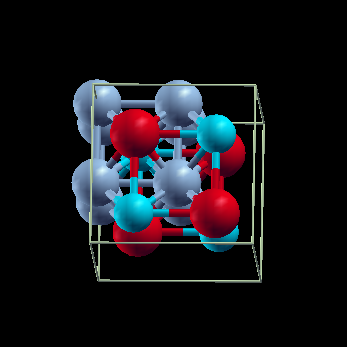
\includegraphics[scale=0.5]{images/co2fesi-cell-2.png}
    \caption{Элементарная ячейка Co$_2$FeSi в кубической решетке. Сиреневым цветом показаны атомы Co, красным Fe, голубым Si.}
    \label{fig:cubic-cell}
\end{figure}

\begin{figure}[h]
    \centering
    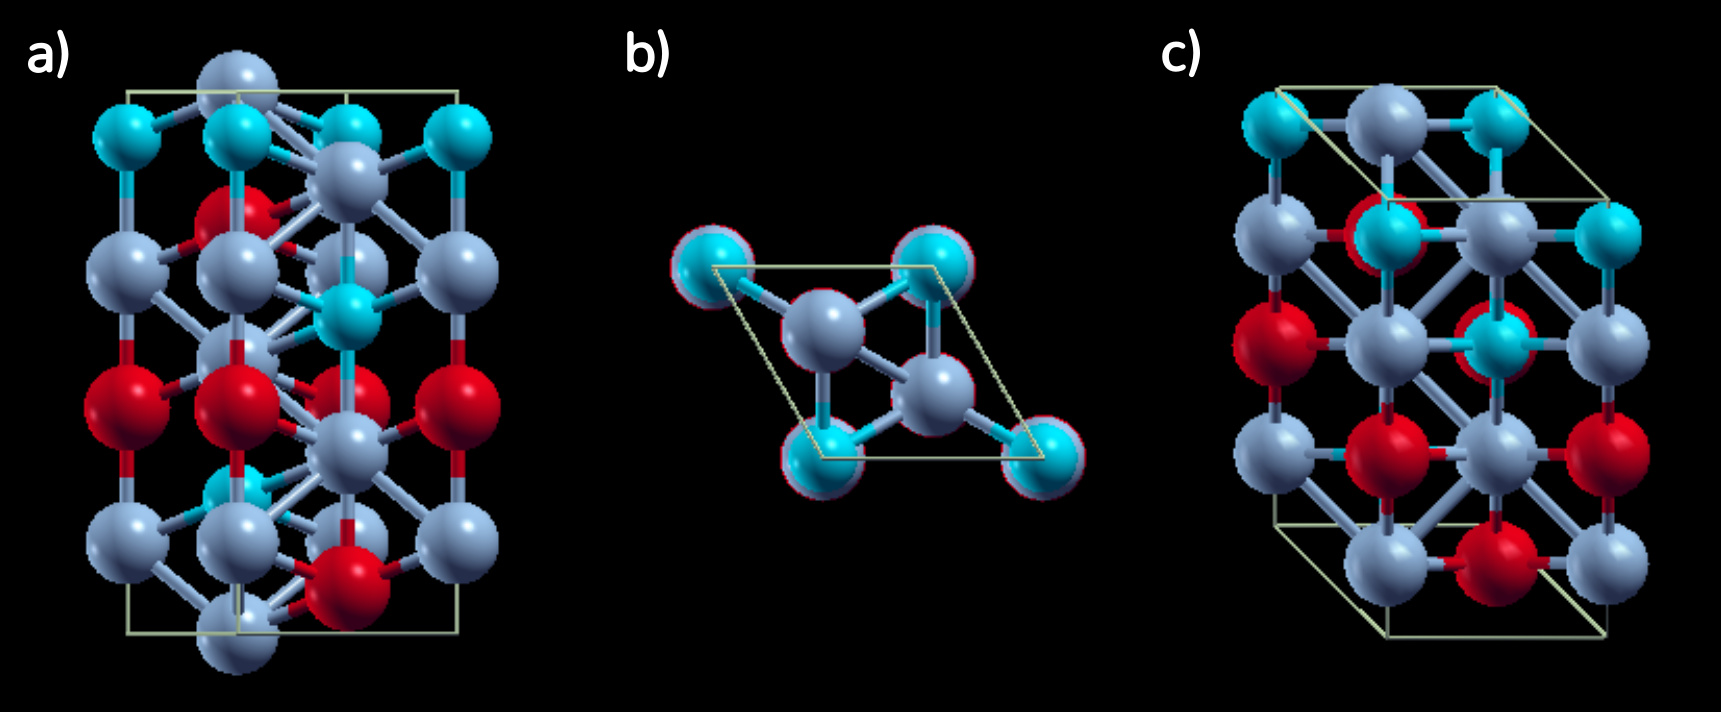
\includegraphics[scale=0.6]{images/hex-cell0.png}
    \caption{Элементарная ячейка Co$_2$FeSi в гексагональной решетке. Сиреневым цветом показаны атомы Co, красным Fe, голубым Si. Приведены изображения сбоку (a), сверху (b), со стороны (с). Сверху находится плоскость (111). }
    \label{fig:hex-cell}
\end{figure}

\begin{figure}[h]
    \centering
    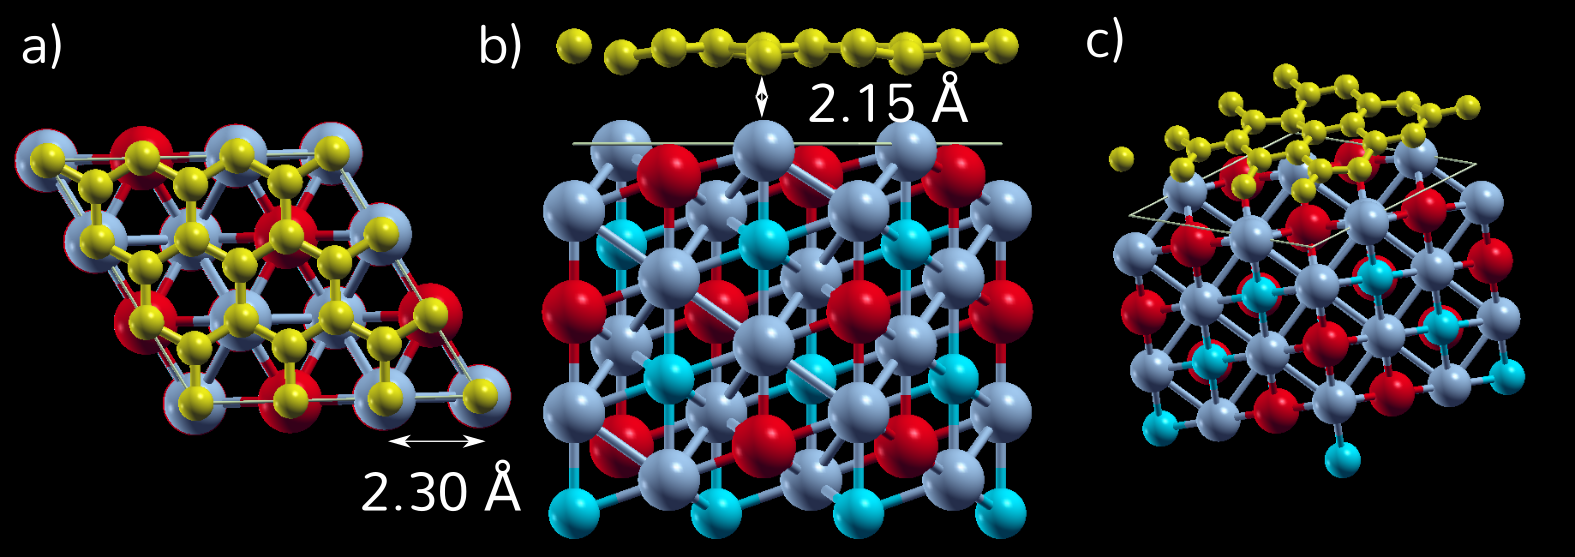
\includegraphics[scale=0.6]{images/co2fesi-graphene-cell.png}
    \caption{Элементарная ячейка Co$_2$FeSi в гексагональной решетке, покрытая графеном. Сиреневым цветом показаны атомы Co, красным Fe, голубым Si, желтым С. Приведены изображения сбоку (a), сверху (b), со стороны (с). }
    \label{fig:graphene-cofe-cell}
\end{figure}

\begin{figure}[h]
    \centering
    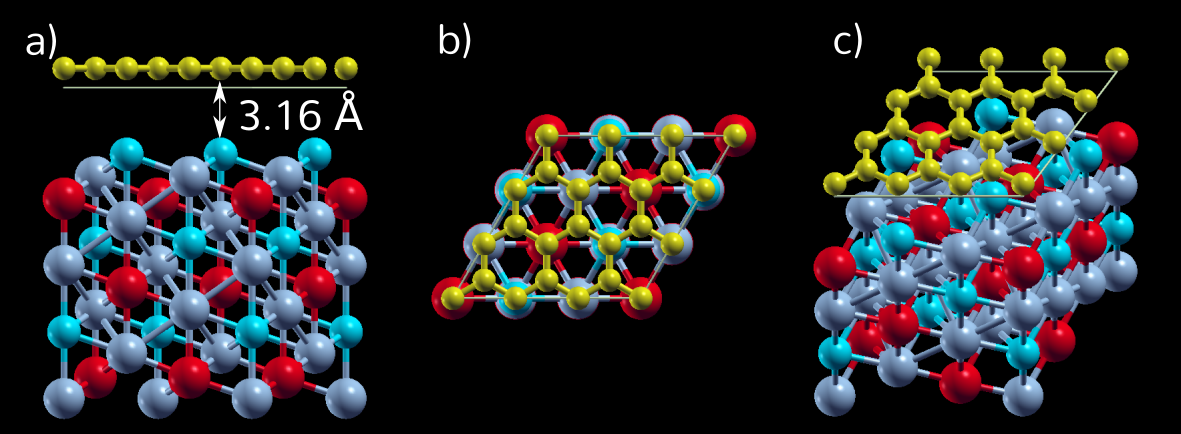
\includegraphics[scale=0.6]{images/sico_cell.png}
    \caption{Элементарная ячейка Co$_2$FeSi в гексагональной решетке, покрытая графеном. Сиреневым цветом показаны атомы Co, красным Fe, голубым Si, желтым С. Приведены изображения сбоку (a), сверху (b), со стороны (с). }
    \label{fig:graphene-cofe-cell}
\end{figure}

\begin{figure}[h]
    \centering
    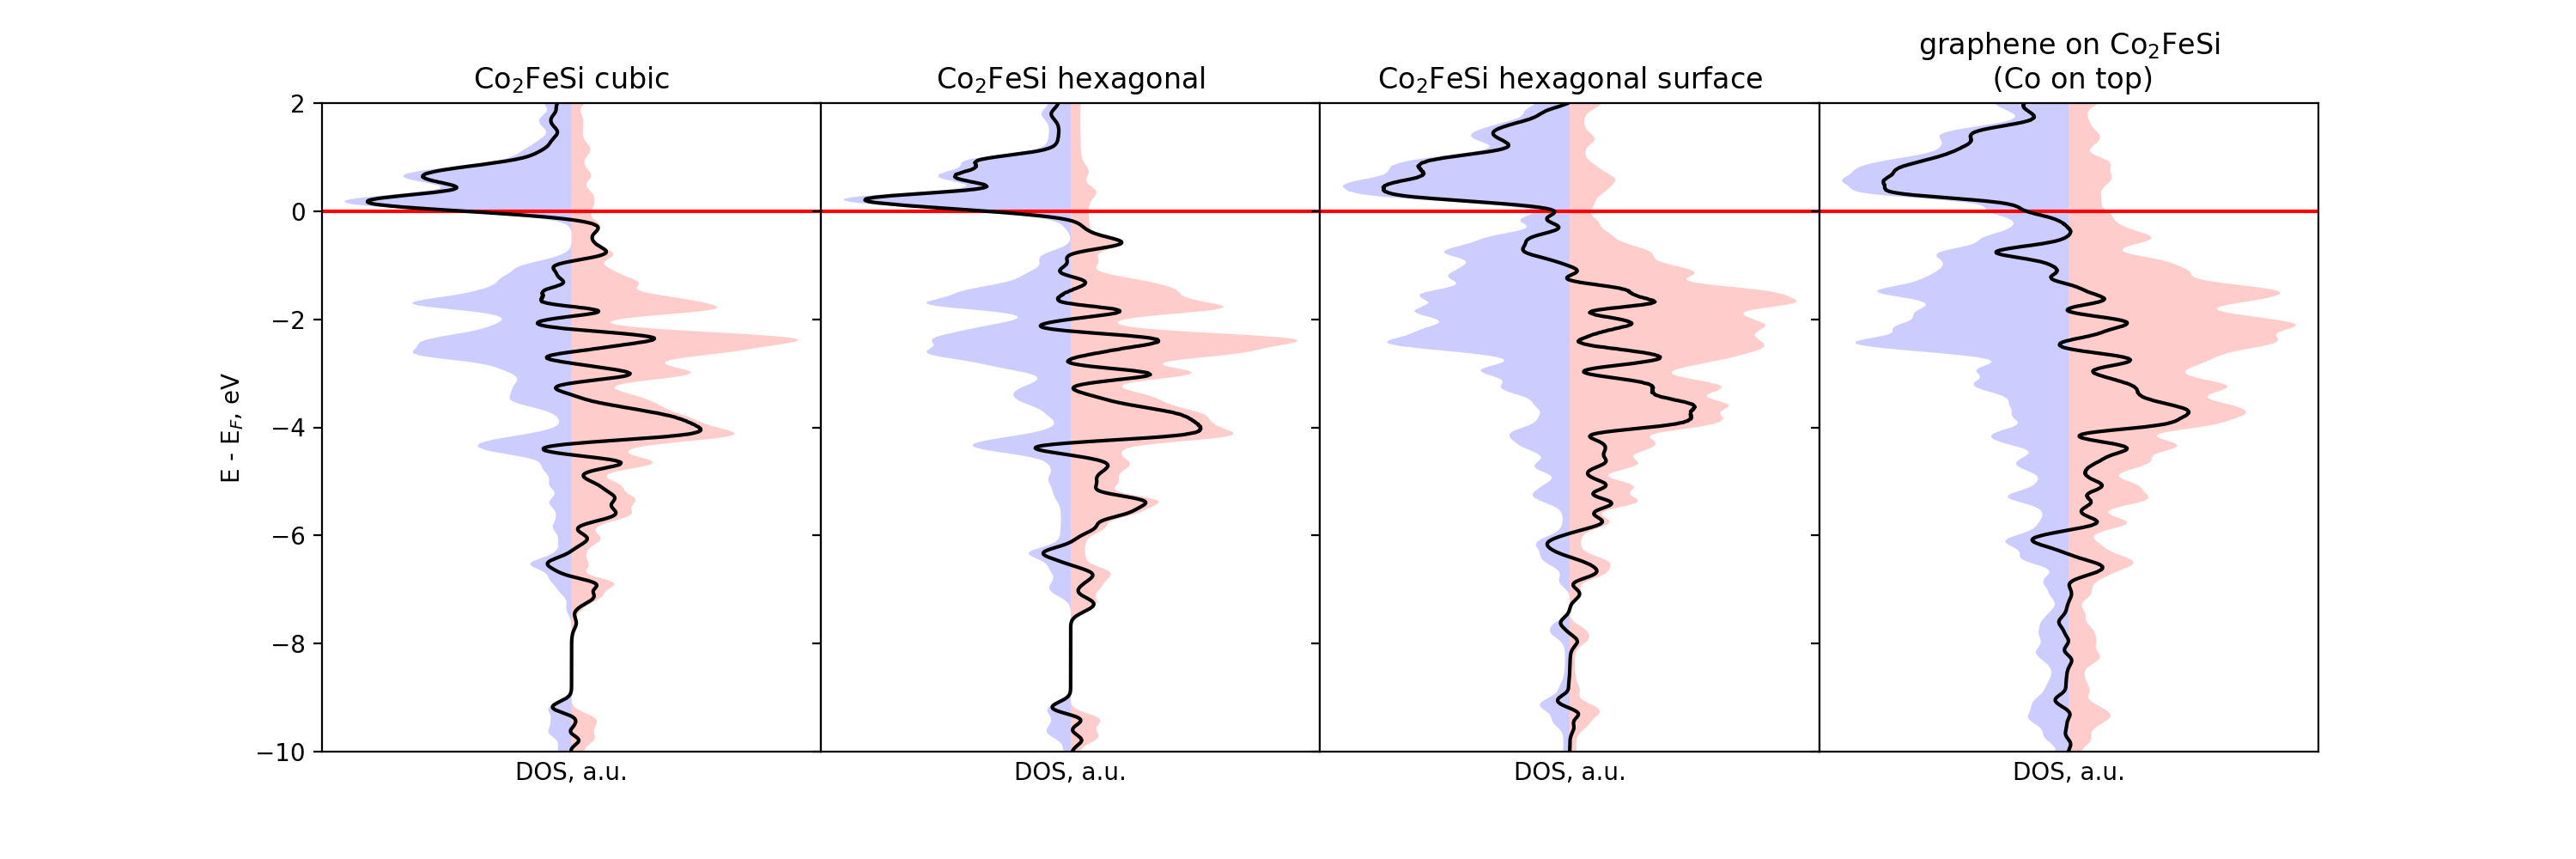
\includegraphics[scale=0.5]{images/070920_dos.png}
    \caption{Плотности состояний Co$_2$FeSi для кубической и гексагональной ячеек, а также для поверхности (111). }
    \label{fig:dos}
\end{figure}

\begin{figure}[h]
    \centering
    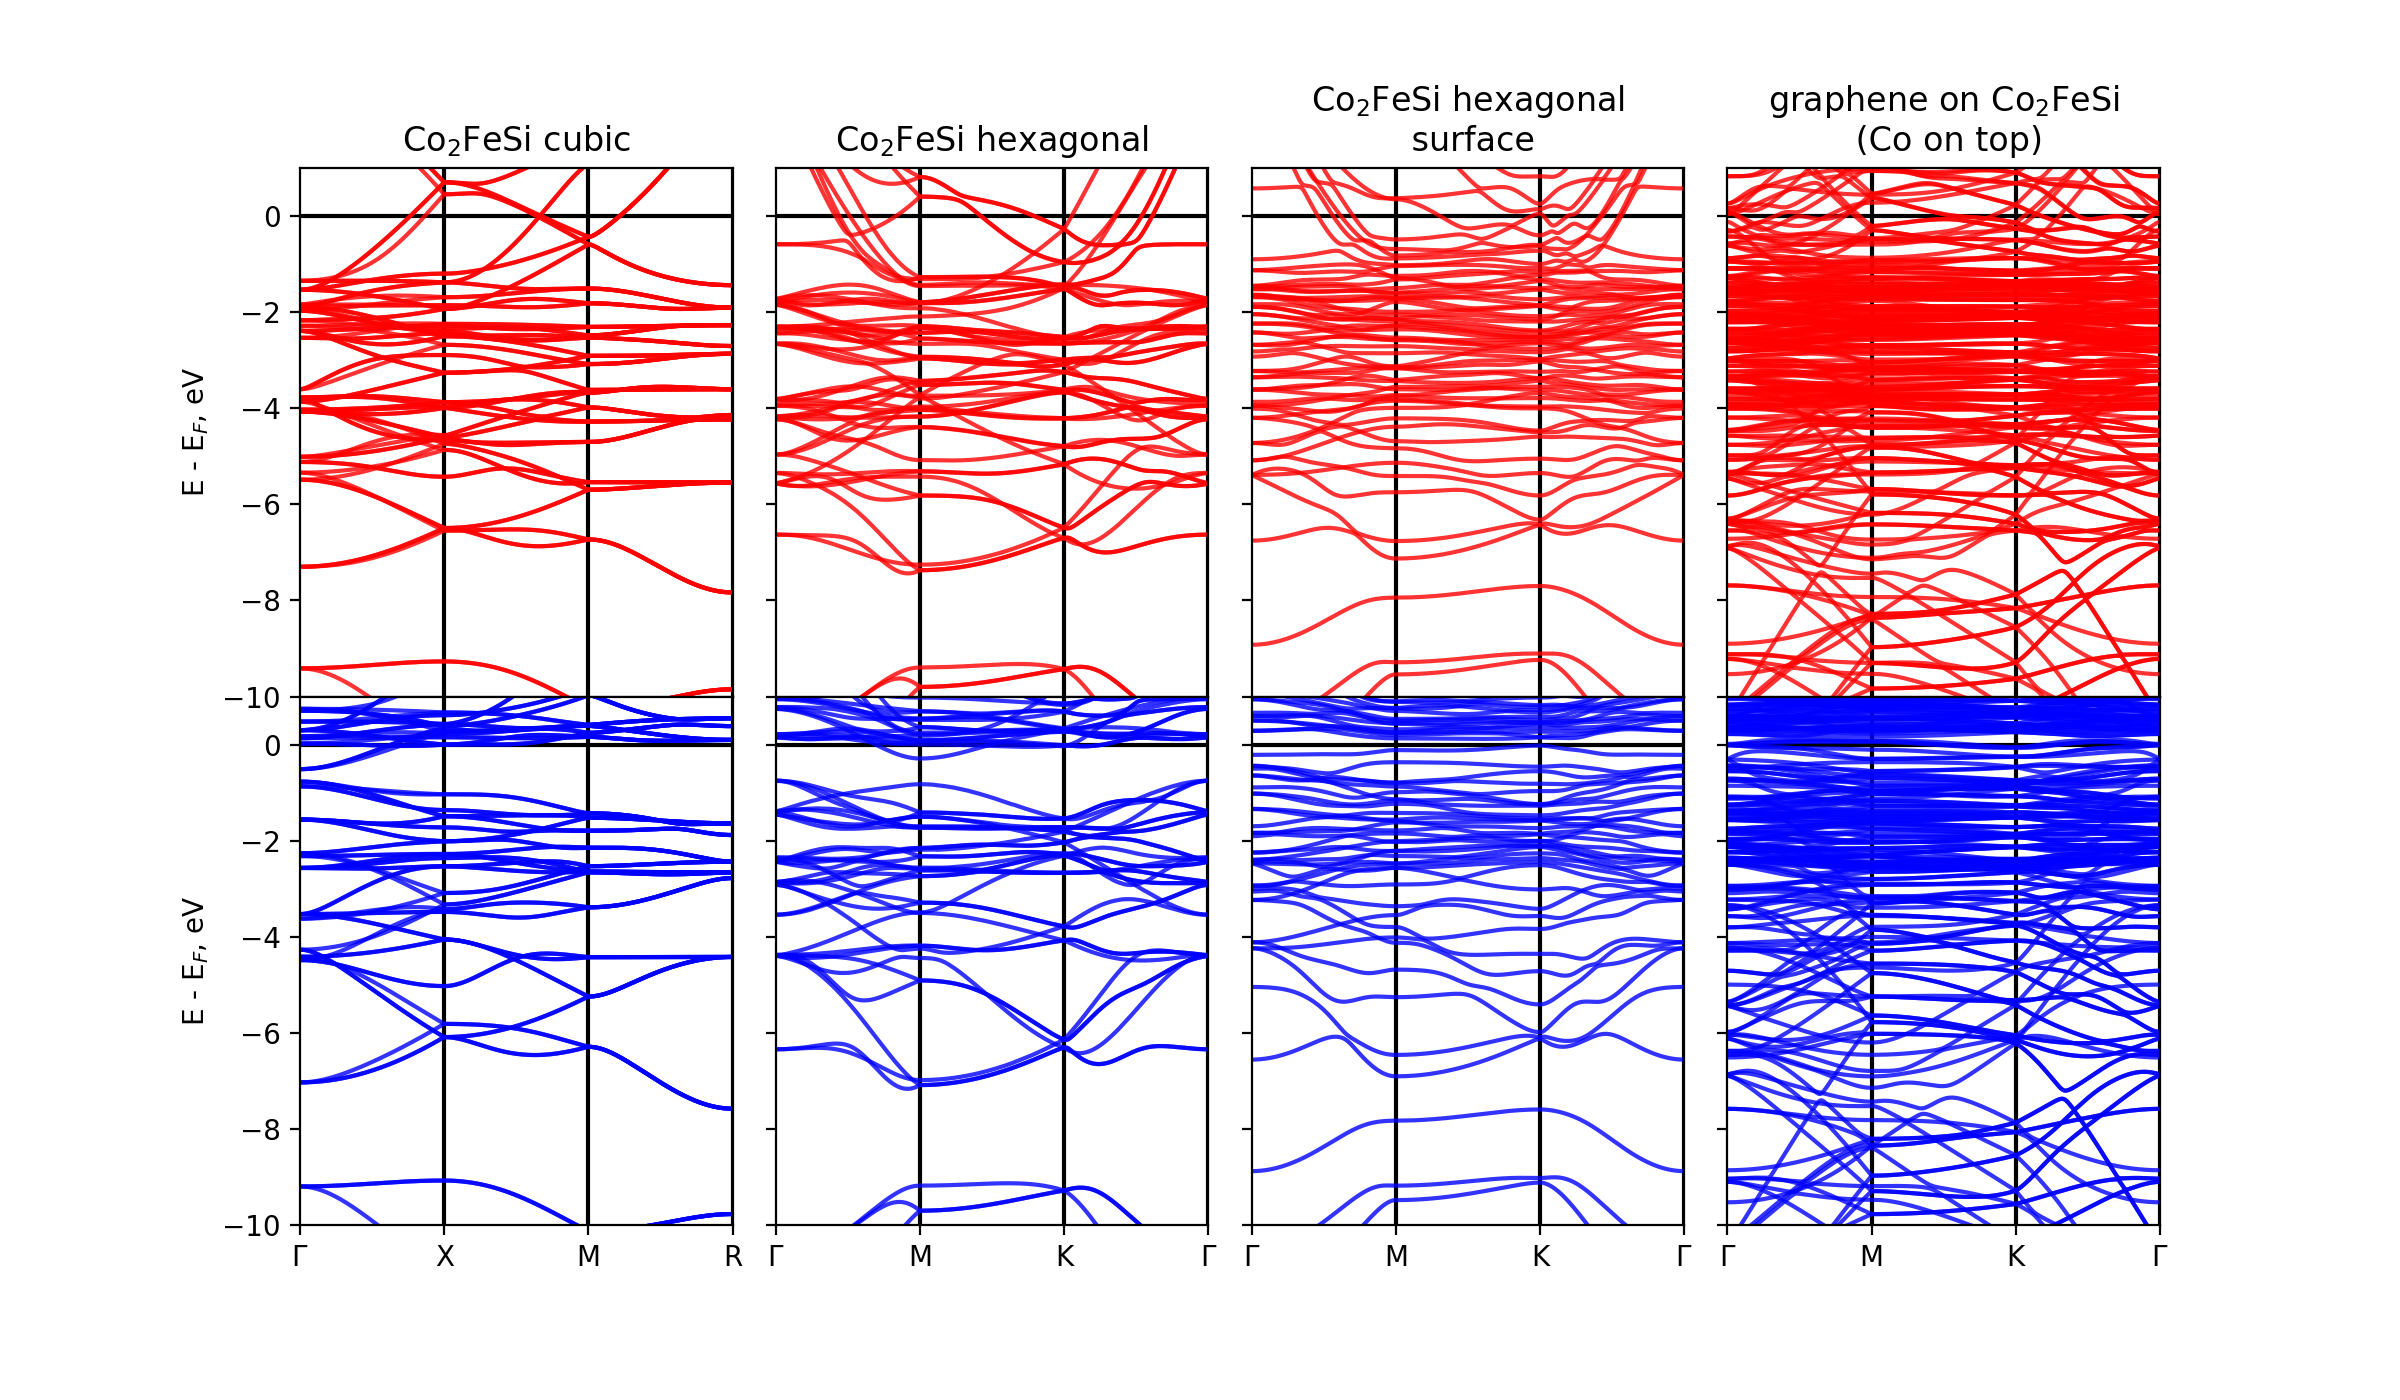
\includegraphics[scale=0.65]{images/070920_bands3.png}
    \caption{Электронная структура Co$_2$FeSi для кубической и гексагональной ячеек, а также для поверхности (111) с графеном и без. }
    \label{fig:bands}
\end{figure}

\begin{figure}[h]
    \centering
    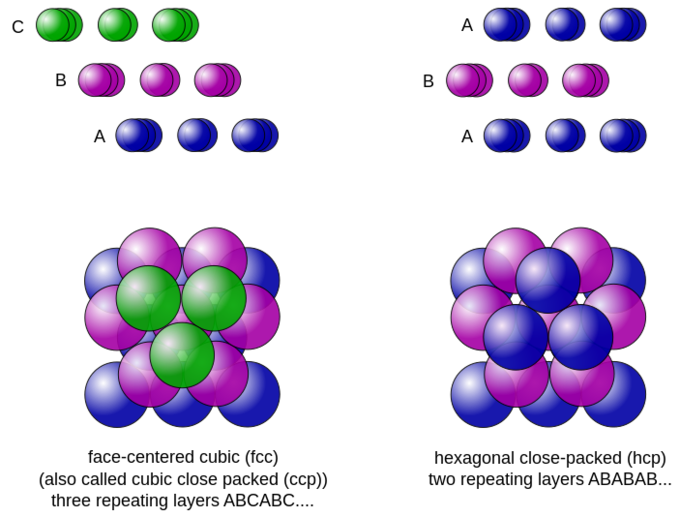
\includegraphics[scale=0.4]{images/Closepacking.svg_.png}
    \caption{Порядок слоев для ГЦК и ГПУ решеток. }
    \label{fig:fcc_vs_hcp}
\end{figure}

\begin{figure}[h]
    \centering
    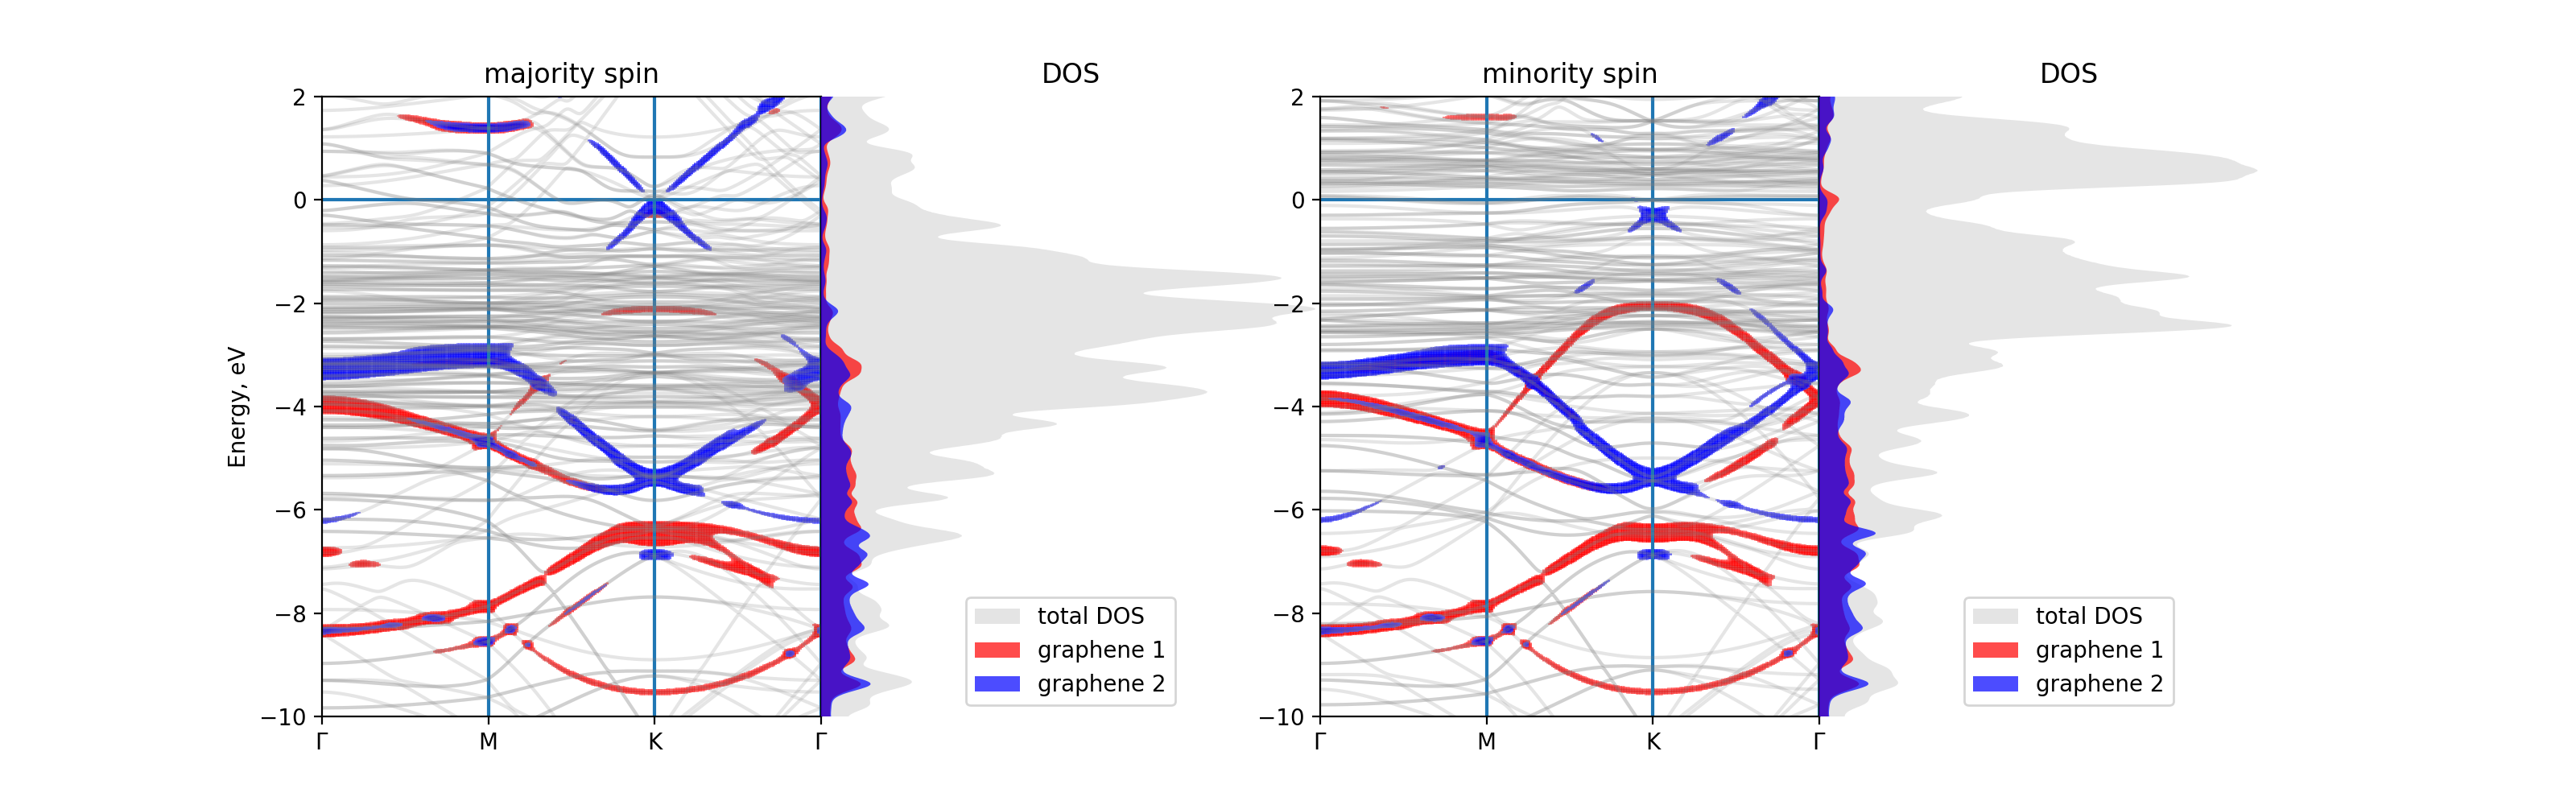
\includegraphics[scale=0.5]{images/co2fesi-graphene00000-100920.png}
    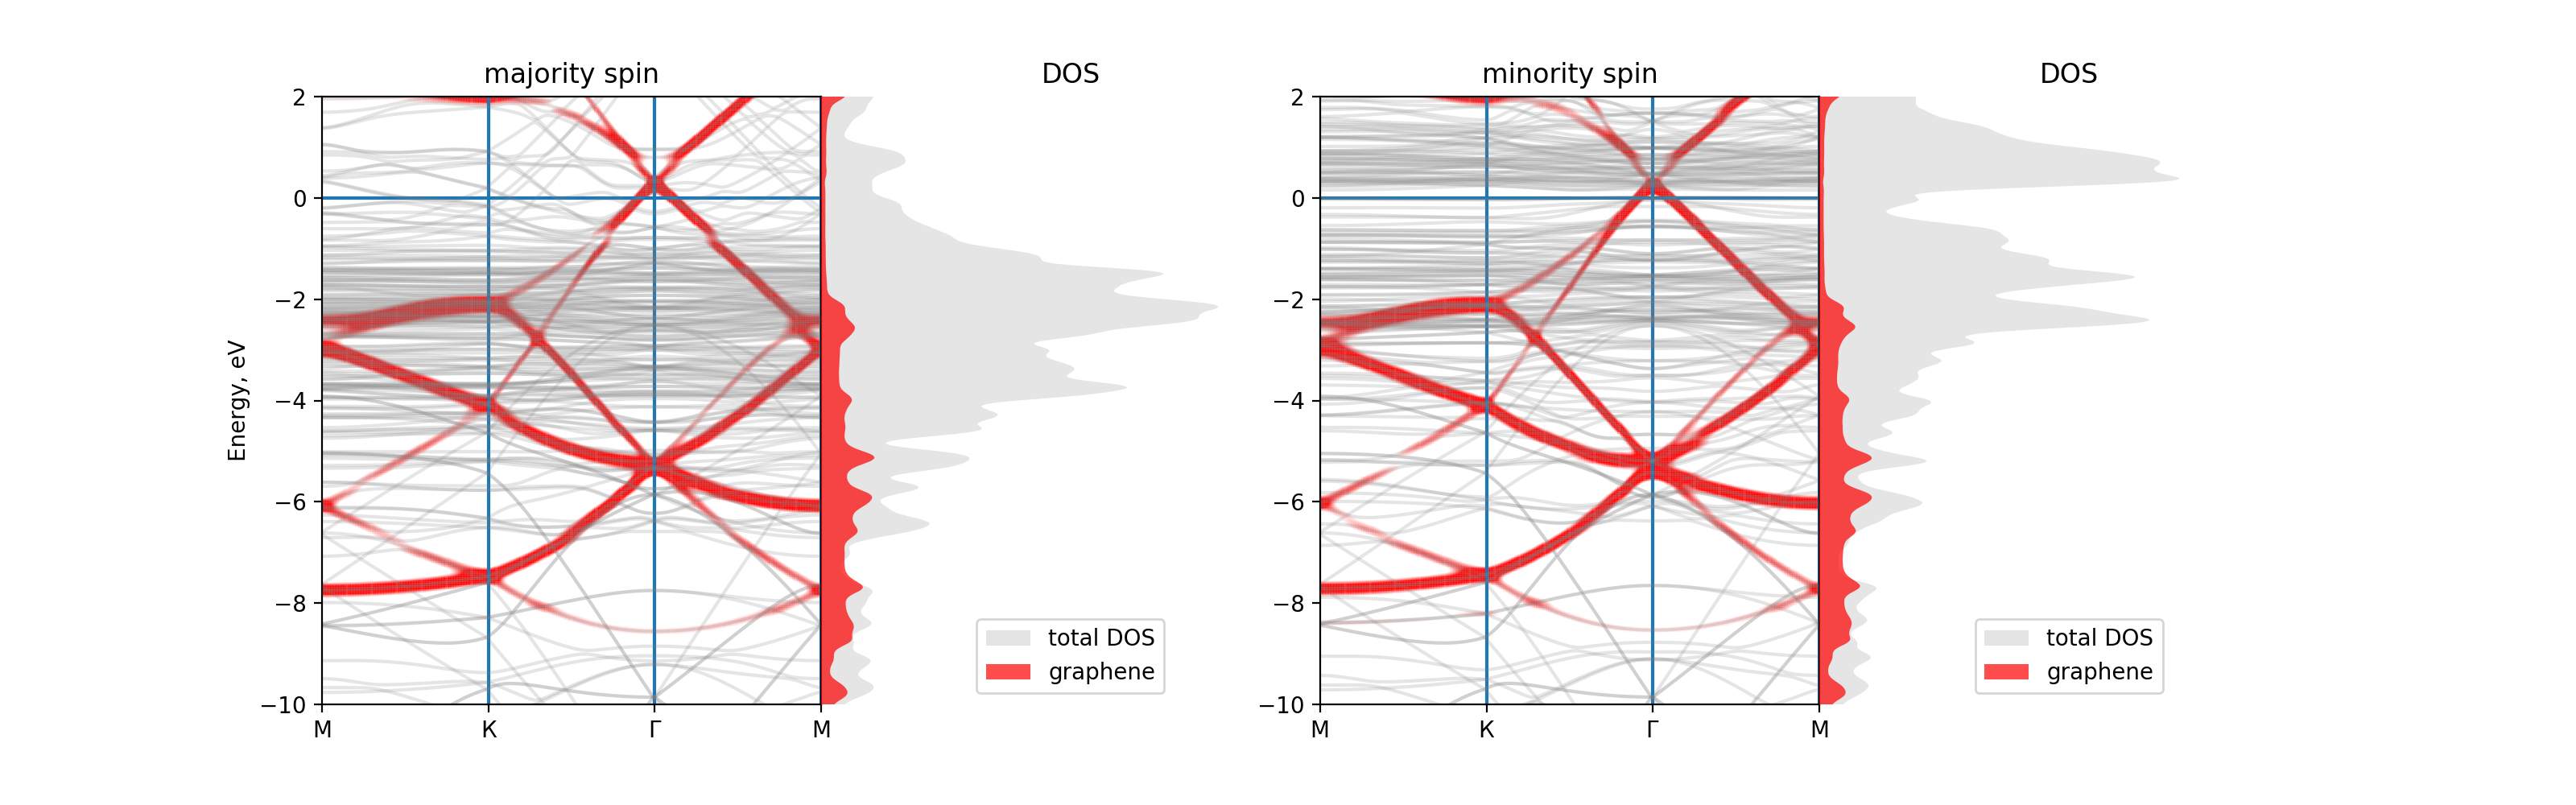
\includegraphics[scale=0.5]{images/co2fesi-graphene-sico2-080920.png}
    \caption{Электронная структура графена на Co$_2$FeSi. Сверху приведен рисунок для графена на кобальтовой грани, снизу - на кремниевой.}
    \label{fig:bands-graphene-cofe}
\end{figure}

\begin{figure}[h]
    \centering
    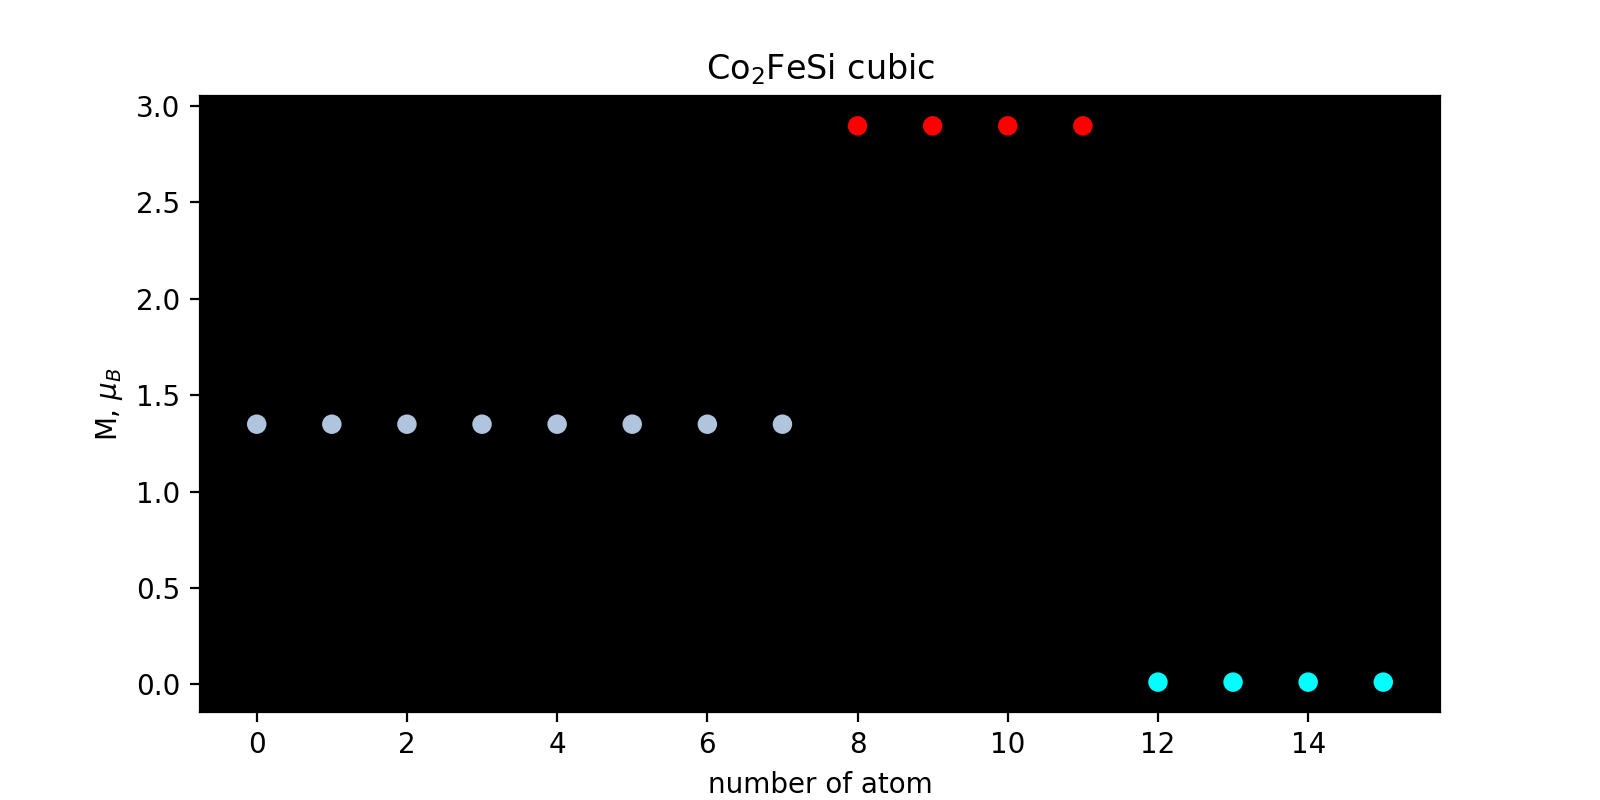
\includegraphics[scale=0.5]{images/co2fesi-cubic-100920_magn_3.png}
    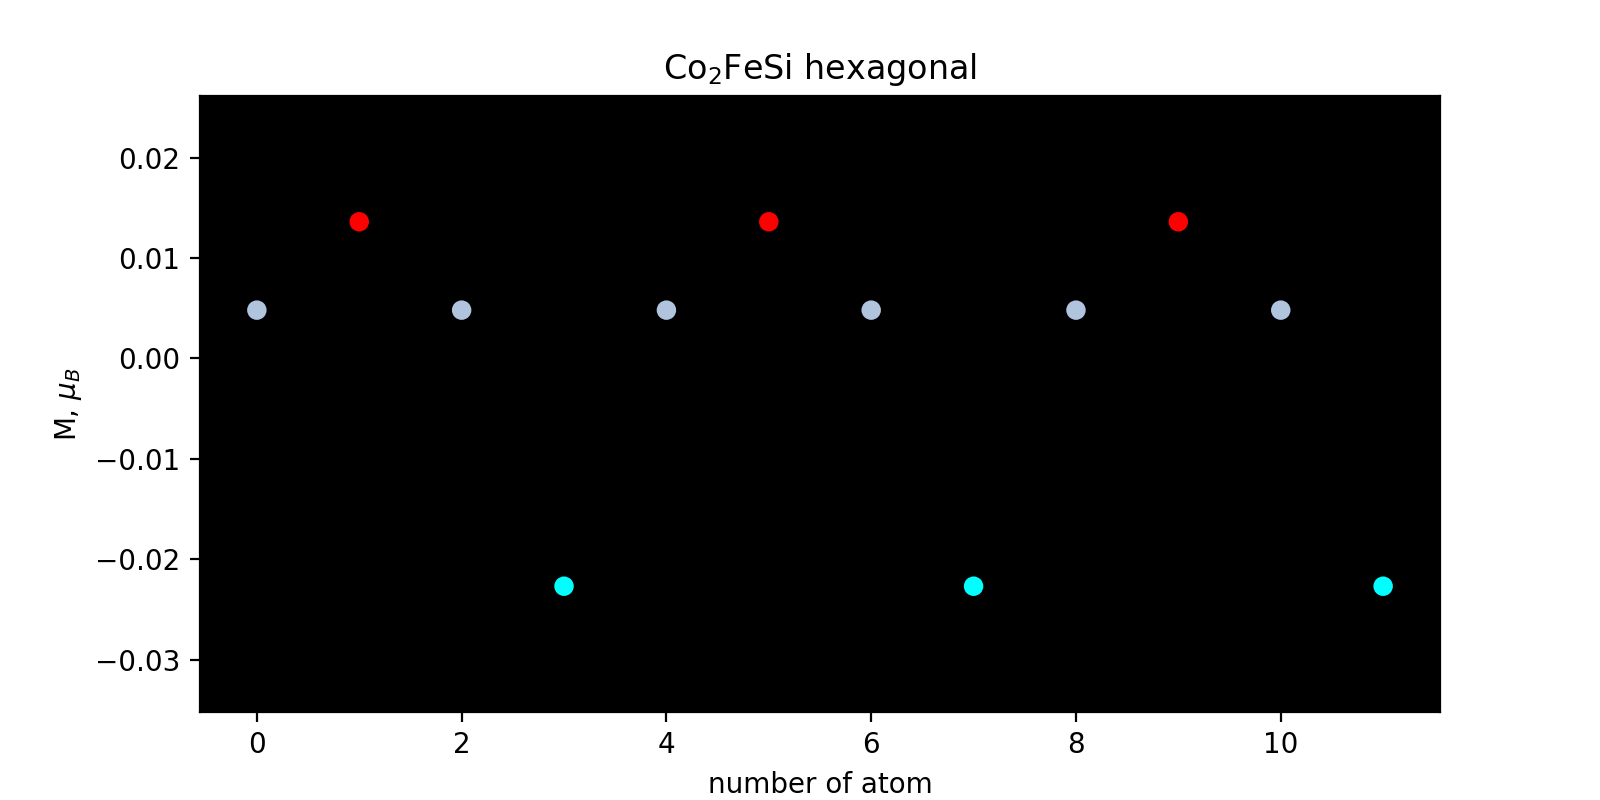
\includegraphics[scale=0.5]{images/co2fesi-hex-100920_magn_3.png}
    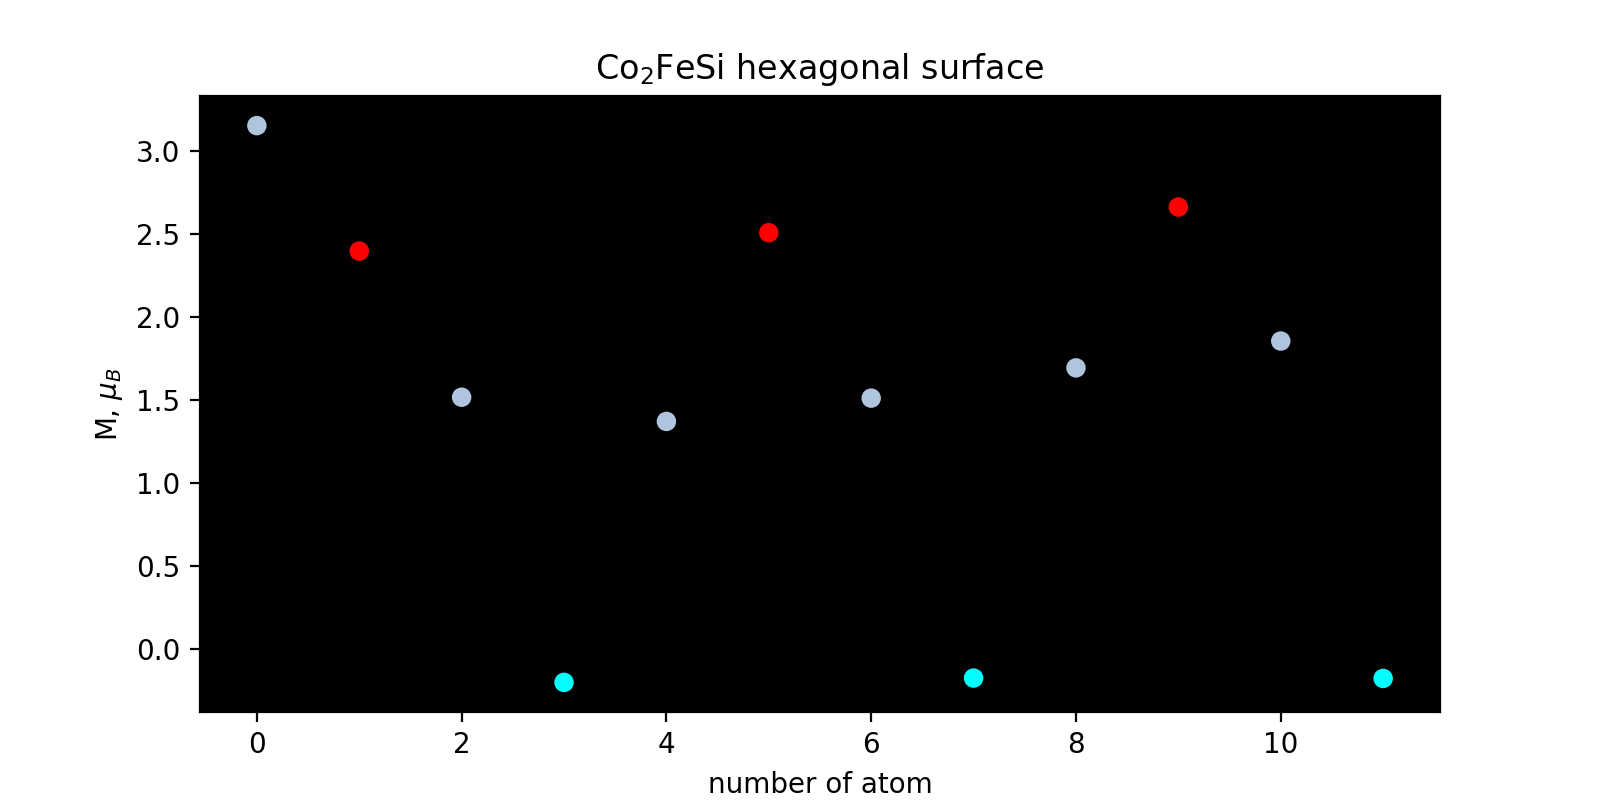
\includegraphics[scale=0.5]{images/co2fesi-hex-surf-100920_magn_3.png}
    \caption{Распределение магнитных моментов в Co$_2$FeSi. }
    \label{fig:magn1}
\end{figure}

\begin{figure}[h]
    \centering
    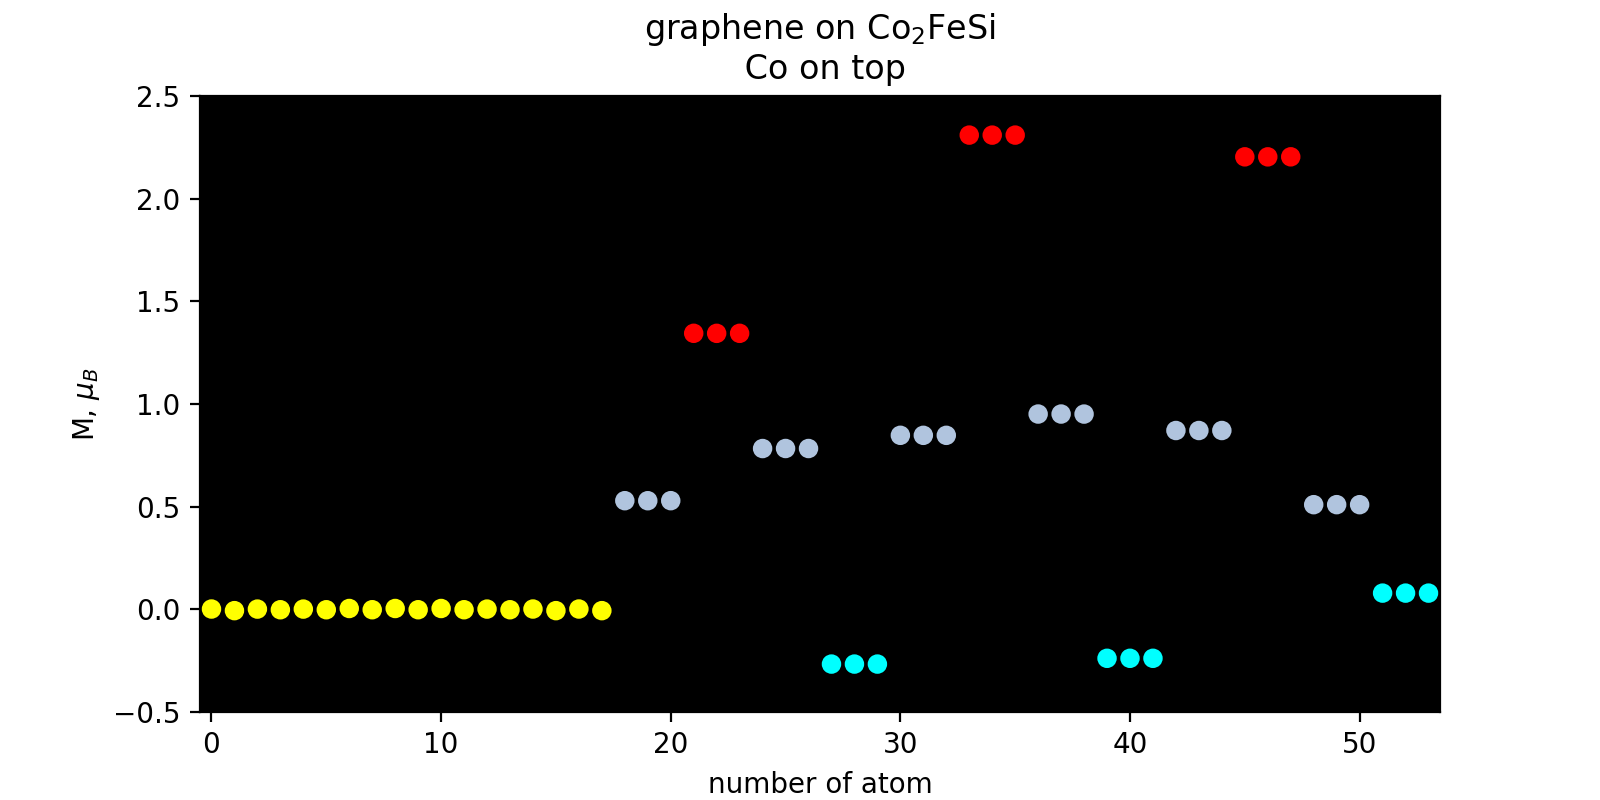
\includegraphics[scale=0.5]{images/co2fesi-graphene-090920_magn_3.png}
    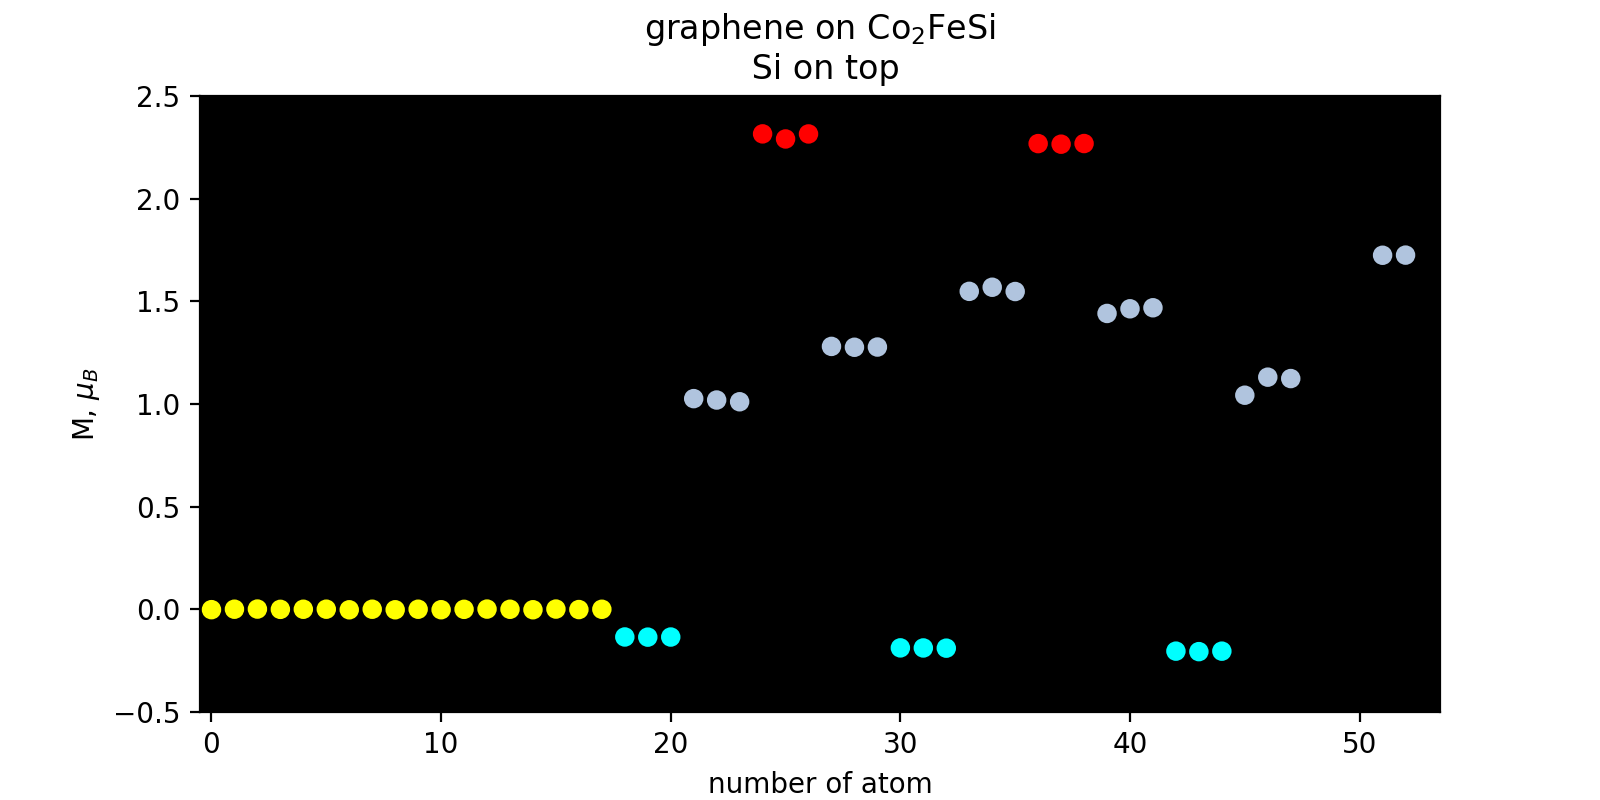
\includegraphics[scale=0.5]{images/co2fesi-graphene-sico-080920_magn_3.png}
    \caption{Распределение магнитных моментов в Co$_2$FeSi, покрытом графеном. }
    \label{fig:magn2}
\end{figure}


\bibliographystyle{unsrt}
\bibliography{cites.bib} 




\end{document}
